\documentclass[11pt]{article}
\usepackage[a4paper,pdftex]{geometry}
\setlength{\oddsidemargin}{5mm}
\setlength{\evensidemargin}{5mm}
\usepackage[english]{babel}
\usepackage{amsmath,amsfonts,amsthm,amssymb}
\usepackage{graphicx}
\usepackage{fancyhdr}
\pagestyle{fancy}
\usepackage{subfig}
\usepackage{wrapfig}
\usepackage{comment}
\usepackage{url}
\usepackage{qtree}
\usepackage{lastpage}
\usepackage{multirow}
\urlstyle{same}
% Page numbering
\lhead{Sentiment Analysis - A Probabilistic Approach}
\rhead{page \thepage/\pageref{LastPage}}
\cfoot{}
\rfoot{\thepage}
% TITLE FORMAT
\newcommand{\HRule}[1]{\rule{\linewidth}{#1}}
\makeatletter
\def\printtitle{
{\centering \@title\par}}
\makeatother									
\makeatletter
\def\printauthor{
{\centering \large \@author}}
\makeatother
% TITLE
\title{
\HRule{0.5pt} \\
\LARGE \textbf{\textsc{Sentiment Analysis}}\\[0.5cm]
\normalsize \textsc{A Probabilistic Approach}
\HRule{2pt}\\ [0.5cm]
\normalsize
\today\\ [4cm]

\includegraphics[width=0.6\textwidth]{titel.png}\\
}
\author{
Supervised by Mr. I. Langbroek (Blauw Research)\\
Mentored by dr. M. van Someren (Universiteit van Amsterdam)\\[0.5cm]
\begin{tabular}{c c c c c}
S. A. Gieske & S. Laan & D. S. ten Velthuis & C. R. Verschoor & A. J. Wiggers\\
6167667 & 6036031 & 0577642 & 10017321 & 6036163
\end{tabular}\\[0.5cm]
Artificial Intelligence\\
Faculty of Science\\
Universiteit van Amsterdam\\
}
% BEGIN DOCUMENT
\begin{document}
% TITLE PAGE
\thispagestyle{empty}
\printtitle									
\vfill
\printauthor
\newpage
% TABLE OF CONTENTS
\setcounter{page}{1}
\normalsize
\tableofcontents
\newpage
% CONTENTS
\section{Introduction}
Due the recent growth of Social Media, such as Facebook, Twitter and blogs, consumers gained a place to review, rate and recommend products online. This online opinion is important for companies who want to market their products, manage their reputations and identify new opportunities. The process of finding relevant content, filtering out noise and categorization of messages can be automated, making it several times faster than manual processing by humans.
Sentiment analysis is the application of natural language processing, computational linguistics and text analytics to identify and extract subjective information in source materials. It readies data from social media for further analysis. By performing sentiment analysis, messages can be clustered into categories (e.g. positive, negative and neutral messages).
\section{Problem Specification}
The supervisor, Ivo Langbroek, provided a spreadsheet of 10.000 messages from social media \footnote{ Data contained posts from Blogs, Facebook, Hyves, fora and tweets}. All messages were manually placed into 5 categories, ranging from very negative to very positive. The goal of this project is to create a method to classify these messages automatically. Before classification the contents of a message needs to be prepared. This is done by cleaning, manipulating and reducing the features inside a message. The preparation of data is described in the following sections.
\subsection{Data Cleaning}
A tweet can contain only 140 characters. Therefore, consumers express themselves by using slang and emoticons. It is also common to find spelling errors in the messages. This results in more noise in the data and therefore it will be important to clean the data. Punctuation usually does not add to the sentiment of the message. Therefore, all punctuation except exclamation marks and question marks are ignored. These two do give value to the sentiment of a sentence as they illustrate the meaning of the emotion used by the consumer. The emotion can also be illustrated with use of emoticons, which consists of various punctuation marks. Emoticons will be substituted for special words to maintain their contribution to the sentiment of a sentence.
A Dutch stemmer, found in the Natural Language Processing Toolkit (NLTK)\footnote{http://www.nltk.org/} for Python, enables reducing inflected words to their stem, the base or root form. For example the words `Evangelisch’ and `Evangelische’ are two words, which lead to the same feature as they are related to each other. By stemming `Evangelische’ into its base form `Evangelisch’, the amount of unique words within the corpus is decreased. This increases the performance of classification as the algorithms have to process less data.
\subsection{Data Reduction}
The dataset consists mostly out of tweets. These short messages contain a single subject, whereas blog and Facebook posts are in general longer messages that may contain several opinions about several subjects. As Twitter is the largest source of information, the classification algorithms implemented are based on these type of posts.
There are several methods to further decrease the vast amount of data:
\begin{itemize}
\item Remove words that occur only once in the corpus.
\item Remove duplicate messages.
\item Remove words that do not contribute to classification such as personal pronouns, stop words, and prepositions.
\end{itemize}
The efficiency of above named methods varies per machine learning method, for example, an approach that considers grammar to be an important feature for classification makes it impossible to remove words from a sentence without affecting the results.
\section{Theory}
%Neural Network, Naive Bayes, MaxEnt, Perceptron
%Relevant Literature is niet nodig volgens Maarten
%\subsection{Relevant Literature}
\subsection{Machine Learning}
Machine Learning is a branch in the field of Artificial Intelligence (AI) that researches and develops algorithms capable of improving predictions or behaviours based on a dataset. An algorithm can take example data to capture the pattern in the underlying probability distribution. A successful algorithm can automatically find these complex patterns in the training data and make intelligent decisions in new similar data. The type of machine learning methods that are used in this assignment is called `supervised learning'. This type requires that the desired prediction, in this case, the sentiment of the messages, is already known.
%tod do: uitleg over verschillende soort machien learning (supervised unsupervised reinforcement etc)
\subsubsection{Perceptron}
A perceptron is an example of a supervised learning algorithm. A perceptron is an artificial neuron, which consists of has one or more inputs $s_i$ with corresponding weights $w_i$, a threshold function $t$ and an output $o$. This output can be defined as $o = t(\sum_i(w_i * s_i))$. The algorithm that enables `learning' a correct threshold takes the following number of steps:
\begin{enumerate}
\item Select training data from the dataset: input and the corresponding (correct) output
\item Feed the perceptron the input
\item Calculate the output
\item Compare the output to the desired output
\item Adjust weights and go to step 2 until satisfied
\end{enumerate}
This algorithm adjusts the weights $w_i$, trying to maximize the number of correct outcomes. It should be noted that a perceptron has only a single output, making it hard to perform Multiclass Classification, when there is more than one class. For multiclass classification other algorithms can be used like the Artificial Neural Network, which is the Multiclass variant of the perceptron and described in the following section.
\subsubsection{Artificial Neural Network}
An Artificial Neural Network (ANN) is a computational model with the same functional aspects as biological neural networks. It consists of a group of connected artificial neurons and changes structure based on internal and external information. The neurons are similar to perceptrons, the only difference being that an output of one neuron can be the input for another. A typical network consists of an input layer, one or more hidden layers and an output layer. The number of nodes per layer can vary. The learning process is very similar to that of a perceptron but is slightly more difficult since the weights are not independent.
\subsubsection{Naive Bayes Classifier}
The Naive Bayes Classifier classifies a sentence using Bayes theorem:
\begin{equation}
P(A|B) = \frac{P(B|A)P(A)}{P(B)}
P(A|B_1 \dots B_n) = \frac{P(B_1|A)\dots P(B_n) P(A)} { P(B_1 \dots B_n }
\end{equation}
Naive Bayes is naive in the sense that it assumes all features to be independent, i.e. the occurrence of one feature is not correlated to the occurrence of another.
To calculate the probability of a sentence for a certain class, the conditional probabilities of the features are needed. In order to get these probabilities for all the features, all occurrences of the features are counted. If a feature has not occurred in the training set, a count of one is used\footnote{This is called add-one smoothing. Other smoothing methods do exists, but were not tried.}.
All of the conditional probabilities are multiplied together. Now the prior probability of the class is needed. This is the probability it belongs to that class when all features are ignored, i.e. the size of the class in respect to training class. A last multiplication with the prior probability gives the probability for the specified class. Note that we can forget the denominator, as they are all the same for each class.
\subsubsection{Maximum Entropy}
An Maximum Entropy algorithm can automatically extract a set of relationships inherent in the trainingdata and then combine these relations into a model. The idea behind Maximum Entropy models is that one should prefer the most uniform models that satify a given constraint. Max Entropy models are feature-based models. Unlike Naive Bayes, Max Entropy makes no assumptions about the relationships between features, and so might potentially perform better when conditional independence assumptions are not met. This means we can add features like bigrams and phrases to Max Entropy without worrying about features overlapping.
%Voorbeeld formule?
\subsubsection{Weighted Probability Sum}
This method is a variation on the classic Naive Bayes classifier in that it calculates the probability for a sentence to belong to a certain class by the sum of its elements, e.g. the probability that the sentence `Ik hou van de eo' contains a positive sentiment can be defined as the sum of the probabilities of the words `Ik', `hou', `van', `de' and `eo' to contain positive sentiment. Mathematically, this looks like:
$\displaystyle P(s, C) = \sum_{i=0}^n P( s[i], C )$, where $C$ is the class, $s $ is the sentence and $s[i]$ is the $i^{th}$ element of s.
This approach uses each word in the sentence as a feature. It is however possible to take $n$ words as a feature, called an $n$-gram. A sentence of length $l$ where $n \leq l$ words contains $l - (n-1)$ sequences of $n$ words. Negations can be included for $n \ge 2$, double negations for $n \ge 3$, etc. The use of $n$-grams as well as 1-grams greatly improves the result of the method.
\subsection{Classification Measures}
%Waarschijnlijk deze substecion voor machine learning
In order to test the performance of the algorithms, a couple of measurements are used. Each will be explained briefly using the elements in this table \ref{classification}.
\begin{table}[h]
\center
\begin{tabular}{cc|c|c|}
\cline{3-4}
& & \multicolumn{2}{|c|}{Classified Class} \\ \cline{3-4}
& & Positive & Negative \\ \cline{1-4}
\multicolumn{1}{|c|}{\multirow{2}{*}{Actual Class}} &
\multicolumn{1}{|c|}{Positive} & TP & FN \\ \cline{2-4}
\multicolumn{1}{|c|}{} &
\multicolumn{1}{|c|}{Negative} & FP & TN \\ \cline{1-4}
\end{tabular}
\caption{Table of classification classes}
\label{classification}
\end{table}
\subsubsection{Accuracy}
The accuracy of a method is a measure of how much correct classifications took place = $\frac{TP+TN}{TP+FP+FN+TN}$.
\subsubsection{Precision}
Precision represents the measure of how many items that are classified as relevant (positive) are actually positive. It is defined as follows:
\begin{equation*}
\textit{Precision} = \frac{ \textit{TP}}{\textit{TP} + \textit{FP}}
\end{equation*}
\subsubsection{Recall}
Recall represents the measure of how many relevant items are actually classified as positive. It is defined as follows:
\begin{equation*}
\textit{Recall} = \frac{ \textit{TP}}{\textit{TP} + \textit{FN}}
\end{equation*}
For this assignment, recall (or precision, based on the classes) is probably the most important of the three. If sentimental sentences are seen as the ‘positive’ class 1 and non-sentimental sentences as the ‘negative’ class 0, the recall is based on the amount of sentimental sentences from the test set that are actually predicted as being positive class. Low recall would thus mean that the sentimental messages `the relevant data’ are seen as negative and thrown away. However, if non-sentimental messages are class 1 and sentimental message are class 0, the perspective is different.
\section{Usage and User Guide}
In this section the usage of the online classification is described. The online classification service should be used in the following way:
\begin{enumerate}
\item Send a request to www.yourwebhost.com/path/to/service/?\textbf{message}=”De eo is heel cool”\&\textbf{dataset}=1\\
\textbf{Message}: is the message to be classified\\
\textbf{Dataset}: is the number of the dataset to be used.
\item Receive the resulting XML file.
\end{enumerate}
\section{Results and Approach}
In this section the results are presented and discussed found by the various algorithms that have been implemented. This section discusses the following: the results, the global approach, binary classification and real time classification.

\subsection{Naive Bayes Classifier}
This section provides and discusses, the results of the Naive Bayes multi-classification algorithm. There were two implementations of the Naive Bayes Classifier, the self-made implementation and the Natural Language Tool Kit (NLTK) implementation. The implementations gave the following results:\\\\
\textbf{Result table self-made implementation:}\\
\begin{tabular}{| l || c | c | c |}
\hline
\textbf{Message type} & \textbf{Accuracy} & \textbf{Precision} & \textbf{Recall}\\
\hline \hline
\textbf{Positive} & 0.81 & 0.39 & 0.43\\
\hline
\textbf{Negative} & 0.71 & 0.17 & 0.40\\
\hline
\textbf{Neutral}  & 0.59 & 0.79 & 0.61\\
\hline
\end{tabular}\\\\
\textbf{Result table NLTK implementation:}\\\\
\begin{tabular}{| l || c | c | c |}
\hline
\textbf{Message type} & \textbf{Accuracy} & \textbf{Precision} & \textbf{Recall}\\
\hline \hline
\textbf{Positive} & 0.80 & 0.34 & 0.42\\
\hline
\textbf{Negative} & 0.72 & 0.18 & 0.40\\
\hline
\textbf{Neutral}  & 0.58 & 0.79 & 0.60\\
\hline
\end{tabular}\\\\\\
\textbf{Conclusion}\\
The Naive Bayes multi-classification algorithm results in a low recall and precision for the messages containing sentiment. This is the case for both implementations eventhough the self-made implementation performs beter, than the NLTK implementation. Therefore, it is not a suitable classification algorithm to solve the sentiment analysis problem.

\subsection{Weighted Probability Sum}
This section provides and discusses, the results of the Weighted Probability Sum binary-classification algorithm. The algorithm gave the following results:\\\\
\textbf{Result table Neutral versus Non-Neutral:}\\\\
\begin{tabular}{| l || c | c | c |}
\hline
\textbf{Message type} & \textbf{Accuracy} & \textbf{Precision} & \textbf{Recall}\\
\hline \hline
\textbf{Neutral} & 0.78 & 0.78 & 0.99\\
\hline
\textbf{Non-Neutral} & 0.77 & 0.85 & 0.16\\
\hline
\end{tabular}\\\\\\
\textbf{Result scatter plots Neutral (green) versus Non-Neutral (red):}
\begin{figure}[!h]
\centering
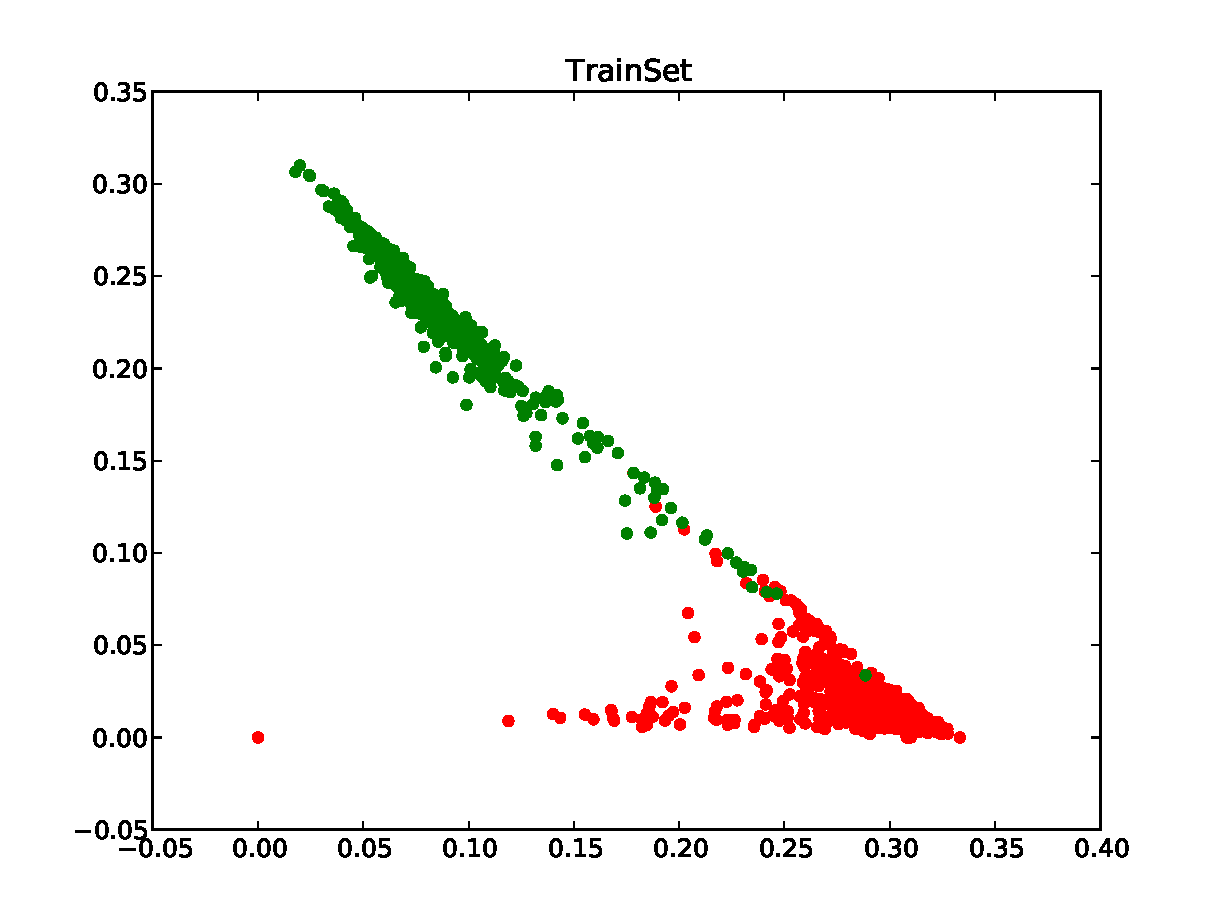
\includegraphics[width=0.4\textwidth]{NeuNonNeuScatter1.pdf}
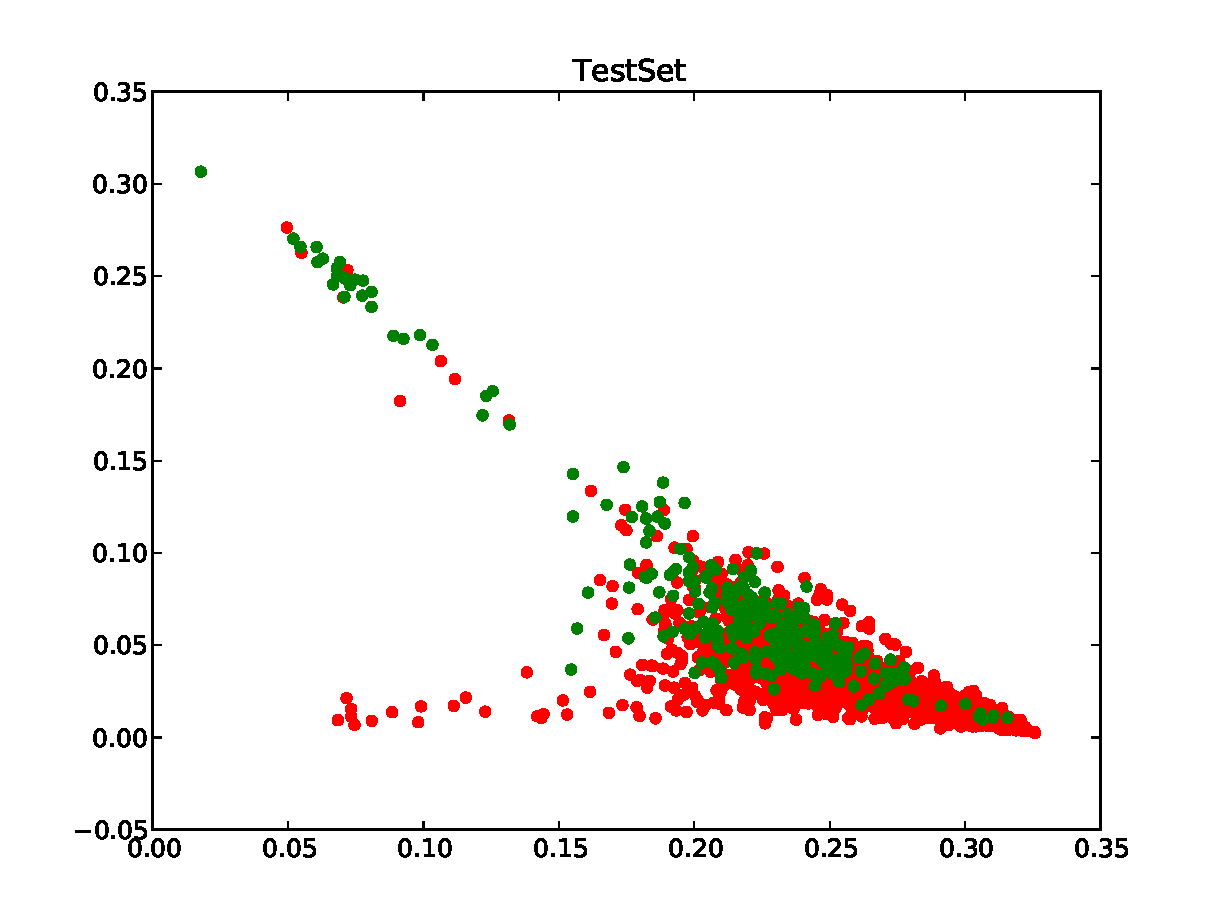
\includegraphics[width=0.4\textwidth]{NeuNonNeuScatter2.pdf}
\caption{Scatter plots of the Training set (left) and Test set (right).}
\label{neunon}
\end{figure}
\newpage
\noindent\textbf{Result table Positive versus Negative:}\\\\
\begin{tabular}{| l || c | c | c |}
\hline
\textbf{Message type} & \textbf{Accuracy} & \textbf{Precision} & \textbf{Recall}\\
\hline \hline
\textbf{Positive} & 0.83 & 0.93 & 0.76\\
\hline
\textbf{Negative} & 0.75 & 0.91 & 0.81\\
\hline
\end{tabular}\\\\\\
\textbf{Result scatter plots Positive (green) versus Negative (red):}
\begin{figure}[!h]
\centering
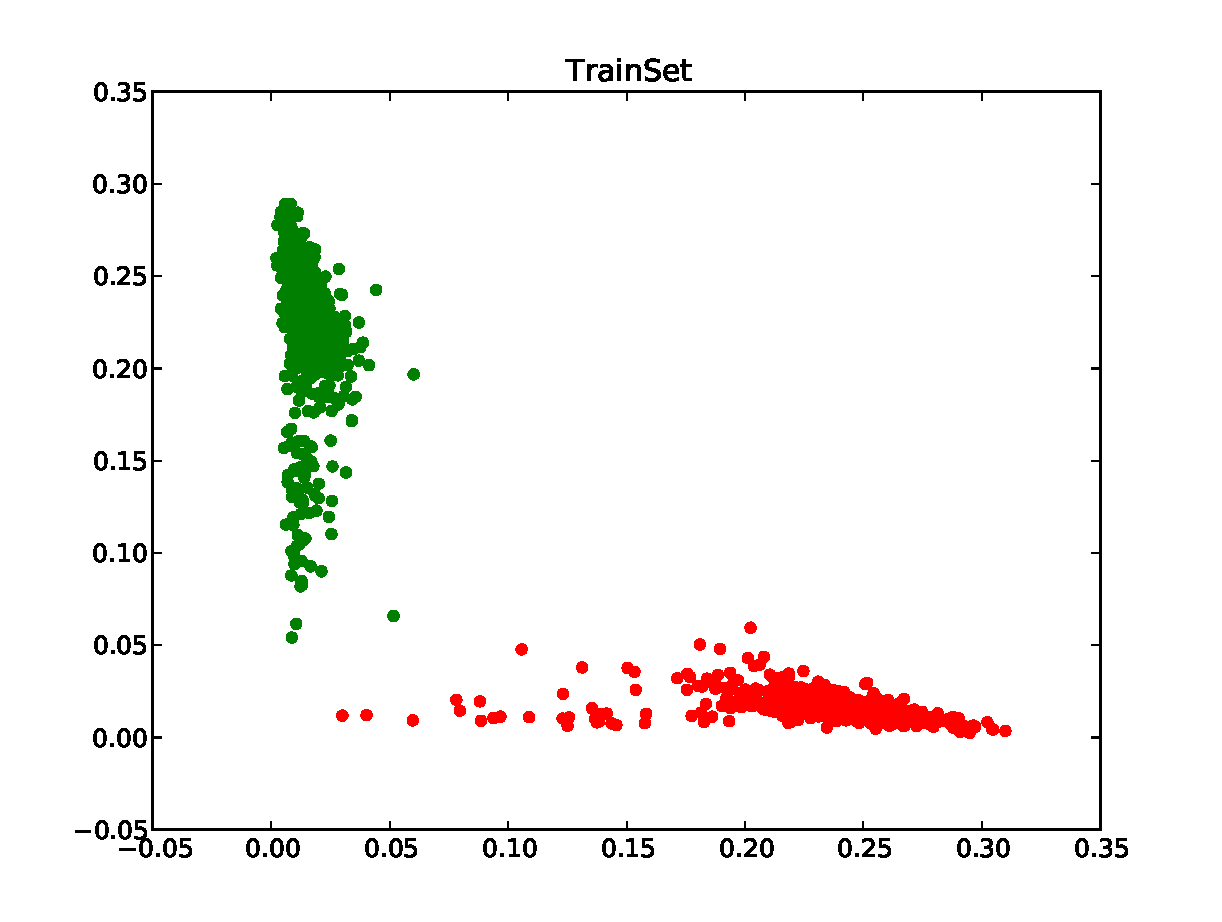
\includegraphics[width=0.4\textwidth]{PosNegScatter1.pdf}
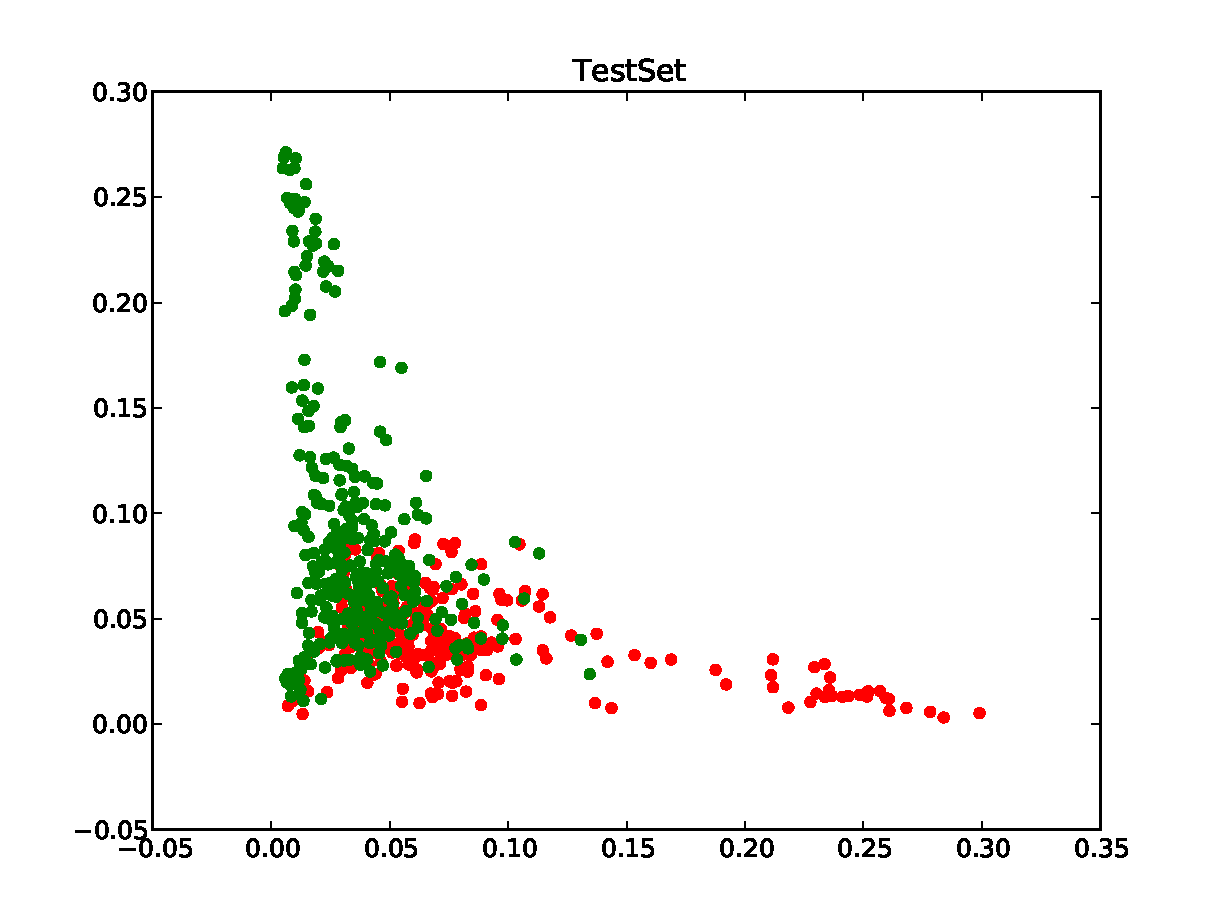
\includegraphics[width=0.4\textwidth]{PosNegScatter2.pdf}
\caption{Scatter plots of the Training set (left) and Test set (right).}
\label{posneg}
\end{figure}

\noindent\textbf{Conclusion}\\
The weighted probability sum performs better, since the probabilities do not get too small. The probabilities of the Naive Bayes approach were so small, that new examples could not be classified correctly: it was no better than guessing. Using the weighted sum approach, the probabilities became not that small. Therefore, a distinction could still be made even with new examples. Figure \ref{neunon} and \ref{posneg} show the probabilities of two classes. In figure \ref{posneg}, the horizontal axis is the probability the tweet is negative, the vertical axis is the positive probability. As you can see this approach is relatively good when it comes to positive versus negative classification.

\subsection{Perceptron}
This section provides and discusses, the results of the Perceptron binary-classification algorithm. In the Weighted Probability Sum algorithm the perceptron was already used to find a threshold. This section only discusses the perceptron with a word vector as input. The algorithm gave the following results:\\\\
\textbf{Result table Neutral versus Non-Neutral:}\\\\
\begin{tabular}{| l || c | c | c |}
\hline
\textbf{Message type} & \textbf{Accuracy} & \textbf{Precision} & \textbf{Recall}\\
\hline \hline
\textbf{Neutral} & 0.77 & 0.79 & 0.95\\
\hline
\textbf{Non-Neutral} & 0.77 & 0.65 & 0.27\\
\hline
\end{tabular}\\\\\\
\textbf{Conclusion}\\
The Perceptron binary-classification algorithm results in a either a low recall or precision for the messages containing sentiment. This means that a linear threshold is not good enough. Therefore, this is not a suitable classification algorithm to solve the sentiment analysis problem.

\subsection{Multi-classification with a Perceptron}
This section provides and discusses, the results of the Perceptron multi-classification algorithm. The algorithm gave the following results:\\\\
\textbf{Result table Positive versus Negative versus Neutral:}\\\\
\begin{tabular}{| l || c | c | c |}
\hline
\textbf{Message type} & \textbf{Accuracy} & \textbf{Precision} & \textbf{Recall}\\
\hline \hline
\textbf{Positive} & 0.77 & 0.65 & 0.26\\
\hline
\textbf{Negative} & 0.65 & 0.62 & 0.31\\
\hline
\textbf{Neutral}  & 0.80 & 0.67 & 0.42\\
\hline
\end{tabular}\\\\\\
\textbf{Conclusion}\\
The Perceptron multi-classification algorithm results in a low recall. This means that a great amount of the messages containing sentiment are thrown away. Therefore, this is not a suitable classification algorithm to solve the sentiment analysis problem.

\subsection{Neural Network}
This section provides and discusses, the results of the Neural Network binary-classification algorithm. The algorithm gave the following results:\\\\
\textbf{Result table Neutral versus Non-Neutral:}\\\\
\begin{tabular}{| l || c | c | c |}
\hline
\textbf{Message type} & \textbf{Accuracy} & \textbf{Precision} & \textbf{Recall}\\
\hline \hline
\textbf{Neutral} & 0.70 & 0.70 & 0.89\\
\hline
\textbf{Non-Neutral} & 0.70 & 0.45 & 0.7\\
\hline
\end{tabular}\\\\\\
\textbf{Conclusion}\\
The Neural Network binary-classification algorithm classifies many messages incorrectly. This might come due to the skewed distribution of the messages. The Neural Network will perform better in classifying, when the dataset is distributed more evenly. Therefore, this still can be suitable classification algorithm to solve the sentiment analysis problem.

\subsection{Support Vector Machine}
This section provides and discusses, the results of the Support Vector Machine binary-classification algorithm. The algorithm gave the following results:\\\\
\textbf{Result table Neutral versus Non-Neutral:}\\\\
\begin{tabular}{| l || c | c | c |}
\hline
\textbf{Message type} & \textbf{Accuracy} & \textbf{Precision} & \textbf{Recall}\\
\hline \hline
\textbf{Neutral} & 0.74 & 0.72 & 0.76\\
\hline
\textbf{Non-Neutral} & 0.74 & 0.45 & 0.16\\
\hline
\end{tabular}\\\\\\
\textbf{Conclusion}\\
The Support Vector Machine binary-classification algorithm results in a low recall. This means that many messages containing sentiment are thrown away in the classifying proces. Therefore, this is not a suitable classification algorithm to solve the sentiment analysis problem.

\subsection{Maximum Entropy}
This section provides and discusses, the results of the Maximum Entropy multi-classification algorithm. The algorithm gave the following results:\\\\
\textbf{Result table Positive versus Negative versus Neutral:}\\\\
\begin{tabular}{| l || c | c | c |}
\hline
\textbf{Message type} & \textbf{Accuracy} & \textbf{Precision} & \textbf{Recall}\\
\hline \hline
\textbf{Positive} & 0.74 & 0.26 & 0.45\\
\hline
\textbf{Negative} & 0.87 & 0.50 & 0.21\\
\hline
\textbf{Neutral}  & 0.69 & 0.80 & 0.76\\
\hline
\end{tabular}\\\\\\
\textbf{Conclusion}\\
The Maximum Entropy multi-classification algorithm results in a low recall and precision for the positive and negative class. Therefore, this is not a suitable classification algorithm to solve the sentiment analysis problem.

\subsection{Global Approach}
In this section the general approach will be explained. The idea is to use a binary classifier, i.e. either true or false, multiple times. This way it is possible to first decide whether a message contains sentiment and then decide between the non-neutral messages whether it is a positive or negative message. This tree structure shows the used approach more clearly:
\begin{figure}[h]
\Tree [.{All messages} {Neutral Messages} [.{Non-Neutral Messages} {Positive Messages} {Negative Messages} ] ]
\end{figure}
As you can see, this approach distinguishes between two classes at a time. This is very convenient because there are a lot of techniques that can discriminate between two classes, whereas multiclass-classifiers are less common.
\subsection{Binary Classification}
In this section, the method that we use to classify a message is described. The approach consists of a few steps:
\begin{enumerate}
\item The counting of word frequencies
\item Calculation of word probabilities
\item Calculation of message probabilities
\item Finding a good threshold
\end{enumerate}
First the frequency of each word, i.e. we count how many times it occurs in the training set, is counted. The number of times the word occurs in the opposite class, is equivalent to the total number of encounters minus the encounters in the first class.
When the frequencies of all words\footnote{All words in the training set} are found, the probability for each word can be calculated. This gives an idea of how likely it is to be encountered in a certain class. The formula for this probability is the following:
\begin{equation}
P(word) = \frac{ \sum word \in C_1}{\sum word \in C_1\cup C_2}
\end{equation}
This means that the probability that a word is in $C_1$, the first class, is the number of times it has been encountered in a sentence, which was tagged to be in $C_1$, divided by the total number of encounters.
Now that all words have probabilities assigned to them, or at least all words in the training set, the probabilities of the sentences can be calculated.
\begin{equation}
P(s) = \frac{1}{n} \sum_{w \in s} P(w)
\end{equation}
Where $s$ is the sentence, $n$ the number of words in the sentence and $w$ a word in the sentence. As follows from the formula, the weighted sum of the word probabilities is used.
Now that every sentence has an associated probability, the real machine learning can begin. The goal is to find a threshold for the probabilities; when a sentence probability is higher than a certain amount, it is classified it as $C_1$, otherwise it belongs to $C_2$.
\subsection{Real Time Classification}
During the process of scraping the messages it is best to do this efficiently by classifying the message immediately. In order to do this efficiently the classification has to be real time. Therefore, saving the resulting configurations of the trained algorithms increases the performance of the classifier. Due to this the algorithms do not have to train during the classification since this is done beforehand. The saved configurations can simply be loaded into the classifier, which speeds up the efficiency of the classifying algorithm. The method currently used is the following:
\begin{enumerate}
\item Beforehand
\begin{itemize}
\item Train the algorithms
\item Save the resulting configurations
\end{itemize}
\item Real time
\begin{itemize}
\item Give the classifier input
\item Process the input
\item Load the configurations into the classifier
\item Classify input
\end{itemize}
\end{enumerate}
The sources of the messages are all online, which means that it’s efficient to do the classification online. Therefore a online service is developed where a message can be inputted by the user. The service classifies the message in real-time and then returns the result to the user. In the current implementation the message is processed by the Hypertext Preprocessor (PHP) and Python. The incoming message is parsed by a PHP script that then calls a Python script. In the Python script the message is processed and classified. After classifying, the Python script returns the result to the PHP script, which generates a XML file containing the results. The process in short:
\begin{equation}
Request \rightarrow Server (PHP/Python) \rightarrow Result (XML)
\end{equation}
\section{Discussion}
The several implemented methods each have their advantages and disadvantages. The most important two are the neural network and the weighted sum probability method, since these two approaches are used in the final classification of opinion vs non-opinion and positive vs negative respectively.
Properties of the neural network:
\begin{itemize}
\item Long training time.
\item Works with relatively small datasets for training.
\end{itemize}
Properties of weighted sum probability method:
\begin{itemize}
\item Better predictions than regular multiclass classification by using the one vs. all-approach.
\item Use of n-grams takes negations into consideration.
\item Needs somewhat larger datasets than neural networks.
\end{itemize}
It should also be noted that these approaches were focused on a single subject. If a more general classifier is needed, the first thing necessary is generalization of data. While domain-specific datasets such as the given one contain keywords that lead to classification (e.g. the word `christen’ often leads to negative sentiment in a sentence in this dataset, this does not have to be the case for other datasets) words such as `leuk’ or `slecht’ should be prioritized. It is, for that reason, possible to create a general-purpose sentiment analyzer, i.e subject independent sentiment classification. This may however decrease the performance, as sentences are often context dependent. To be able to cope with this problem a more sophisticated approach has to be taken. We would suggest to look more into the semantic analysis of sentences, i.e. build a tree representation of the sentence.
\section{Conclusion}
The manual classification process of online messages is more accurate when compared to automatic classification. The problem is that classification time is as important as accuracy, if not more, especially when thousands of messages per hour have to be processed. The methods discussed in this report are only a few approaches to the problem, with quite satisfying results. More data will almost always lead to more correct classifications, but it is also important to make correct predictions when little data is available. Neural networks may be able to do this, more so than any of the other approaches. The weighted sum method, that relies on frequencies, will perform much better when more data is involved. However, simple keywords can be used instead of the entire text to make an estimate of the sentiment in a sentence.
\section{References}
\begin{enumerate}
\item Bo Pang, Lillian Lee, \emph{Opinion Mining and Sentiment Analysis}, Foundations and Trends in Information Retrieval. Volume 2 Issue 1-2, January 2008
\item Ainur Yessenalina, Yejin Choi, Claire Cardie, \emph{Automatically generating annotator rationales to improve sentiment classification}, Proceedings of the ACL 2010 Conference Short Papers, pages 336-341, Uppsala, Sweden, 11-16 July 2010
\item Scot Nowson, \emph{Scary Films Good, Scary Flights Bad. Topic driven feature selection for classification of sentiment}, In TSA '09: Proceeding of the 1st international CIKM workshop on Topic-sentiment analysis for mass opinion (2009), pp. 17-24
\item Ramanathan Narayanan, Bing Liu and Alok Choudhary, \emph{Sentiment Analysis of Conditional Sentences}, Proceedings of the 2009 Conference on Empirical Methods in Natural Language Processing, pages 180-189, Singapore, 6-7 August 2009.
\end{enumerate}
\end{document}
% END DOCUMENT